
%% Beamer poster theme created for Imperial College by LianTze Lim
%% LICENSE: LPPL 1.3
\documentclass[xcolor={table}]{beamer}
\usepackage[size=a0,orientation=landscape,scale=1.55]{beamerposter}
\setlength{\oddsidemargin}{1in}
\usepackage{wrapfig}
\usepackage{amsmath}
\usepackage{tabu}
\usepackage{booktabs}
%\usepackage{subcaption}
\usepackage{subfig}[caption=False]
% \captionsetup[table]{font={stretch=1.2}}     %% change 1.2 as you like

\usetheme{ImperialPoster}
%% Four available colour themes
\usecolortheme{ImperialWhite} % Default
% \usecolortheme{ImperialLightBlue}
% \usecolortheme{ImperialDarkBlue}
% \usecolortheme{ImperialBlack}

\title{Demystifying MMD GANs}
\author{
  \mainauthor{Miko{\l}aj Bi\'nkowski}\Tsup{1}, 
  \mainauthor{Dougal J. Sutherland}\Tsup{2},
  Arthur Gretton\Tsup{2},
  Michael Arbel\Tsup{2}
}
\institute{
  \Tsup{1}Department of Mathematics, Imperial College London, 
  \Tsup{2}Gatsby Computational Neuroscience Unit, University College London\\
  \texttt{\{mikbinkowski,dougal,arthur.gretton,michael.n.arbel\}@gmail.com}
}

\DeclareMathOperator{\D}{\mathcal{D}}
\DeclareMathOperator*{\E}{\mathbb{E}}
\newcommand{\F}{\mathcal{F}}
\newcommand{\h}{\mathcal{H}}
\DeclareMathOperator{\mean}{mean}
\newcommand{\PP}{\mathbb P}
\newcommand{\QQ}{\mathbb Q}
\newcommand{\R}{\mathbb R}
\DeclareMathOperator{\W}{\mathcal{W}}
\newcommand{\X}{\mathcal X}
\newcommand{\Z}{\mathcal Z}
\newcommand{\ZZ}{\mathbb Z}
\DeclareMathOperator*{\argmin}{argmin}
\DeclareMathOperator*{\argmax}{argmax}
\DeclareMathOperator{\mmd}{MMD}
\DeclareMathOperator{\mmdhat}{\widehat{MMD}}

\addbibresource{refs.bib}

\begin{document}
\addtobeamertemplate{headline}{} % Imperial Logo. This is a bit hacky
{
\begin{tikzpicture}[remember picture,overlay] 
\node [shift={(-11cm,-5cm)}] at (current page.north east) {
\includegraphics[height=4.5cm]{Imperial_logo.pdf}}; 
\end{tikzpicture} 
\begin{tikzpicture}[remember picture,overlay]
\node [shift={(11cm,-5cm)}] at (current page.north west) {
\includegraphics[height=11cm]{gatsby.jpg}};
\end{tikzpicture}
}


\begin{frame}{}
\maketitle
\begin{columns}[T, totalwidth=\textwidth]

  \begin{column}{.32\textwidth}
    \begin{block}{Introduction}
      \begin{itemize}
        \item We investigate the training and performance of generative adversarial networks 
              using the Maximum Mean Discrepancy.% (MMD GANs). 
        \item We clarify the situation with 
              bias in GAN loss. %and relation between MMD GAN and Cram\'er GAN.
        \item We propose new measure of GAN performance, %the \emph{Kernel Inception Distance} and 
              and adaptive learning rate scheme for training.
      \end{itemize}
    \end{block}
    \vspace*{-1.2cm}
    \begin{block}{Relation to Wasserstein and Cram\'er GANs} 
      Integral Probablity Metrics (IPMs) form a family of divergences between 
      probability distributions
      \begin{equation}
        \D(\PP, \QQ) = \sup_{f\in\F} \E_{X\sim\PP}f(X) - \E_{Y\sim\QQ}f(Y),
      \end{equation}
      where $\F$ is some class of \emph{critic} functions. 
      \begin{itemize}
        \item{\textbf{Wasserstein distance} is the IPM with $\F$ being the set of 1-Lipschitz functions
          \[  
            \F = \left\{f: \sup\frac{|f(x) - f(y)|}{\|x - y\|}\leq 1\right\}. 
          \]
          Wasserstein GANs approximate this class via critic network, with Lipschitz 
          constraint enforced through weight clipping \citep{wgan} or gradient 
          penalty \citep{wgan-gp}.
        \item \textbf{Maximum Mean Discrepancy (MMD)} \citep{mmd-jmlr} is the IPM 
          where $\F$ is the unit ball in some 
          \emph{Reproducing Kernel Hilbert Space (RKHS)} $\h$ with kernel $k$
          \[ \F = \left\{f: \|f\|_{\h} \leq 1\right\}. \]
          MMD value and the optimal critic are known in the closed form
          \begin{align*}
            MMD(\PP, \QQ) &= \E_{\PP} k(X,X') + \E_{\QQ} k(Y,Y') - 2\E_{\PP,\QQ} k(X,Y),\\
            f^*(t) &= \E_{\PP}k(X, t) - \E_{\QQ}k(Y, t).
          \end{align*}
        }
        \item{
          MMD GANs \citep{mmd-gan}, however, 
          optimize \emph{representation} in the composite kernel 
          \[ k_{\theta}(x, y) = k_{base}(h_{\theta}(x), h_{\theta}(y)). \]
        }
        \item Cram\'er GAN is MMD GAN with \emph{Energy Distance} kernel.
        \item WGAN can be seen as MMD GAN with linear kernel.
      \end{itemize}
    \end{block}
    \vspace*{-1.2cm}
    \begin{block}{Gradient Penalty}
      Extending the idea of \citet{wgan-gp}, we penalize the
      gradient of the witness function 
      \[ Loss^{critic}(\theta) = \widehat{MMD_{\theta}}(\PP, \QQ_{\psi}) + \lambda\E_{\tilde{X}}\left(\|\nabla_{\tilde{X}} f^*(\tilde{X})\| - 1\right)^2. \]
      %where $\tilde{X}$ are drawn between points from $\PP$ and $\QQ_{\psi}$. %$\widehat{MMD}$ is an unbiased MMD estimator.% and $\QQ_{\psi} = G_{\psi}(\ZZ)$ is the generated distribution.
    \end{block}
  \end{column}

  \begin{column}{.32\textwidth}
    \begin{figure}
      \centering
        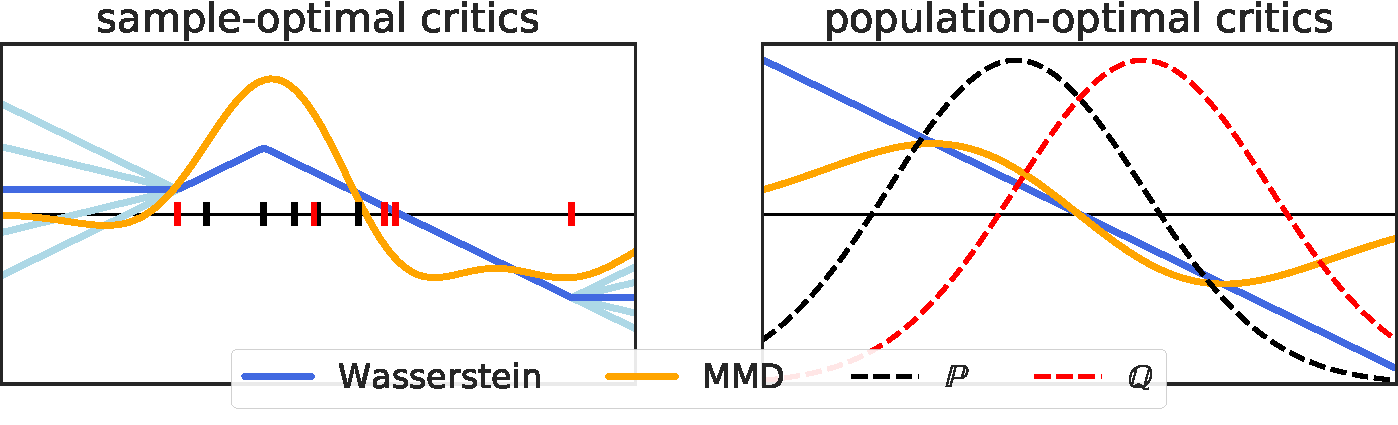
\includegraphics[with=\columnwidth]{witness.pdf}
      \caption{Estimated (left) and population (right) witness functions for MMD and Wasserstein distance between two Gaussians. Note multiple optimal Wasserstein sample witness functions (in light blue).}
    \end{figure}
    \vspace*{-1.3cm}
    \begin{block}{Biased gradient estimates}
      \begin{itemize}
        \item \citet{cramer-gan} claim that WGANs have biased gradients, while Cram\'er GANs do not.
        \item We prove that for Wasserstein, Cram\'er and MMD GANs gradient estimates
              are unbiased, but learning a discriminator based on samples leads to biased gradients 
              for the generator parameters. If $\widehat{\D}$ is the estimate of the loss function: 
        \item $\nabla_{\psi}\widehat{\D}(X, G_{\psi}(Z))$ is biased,
        \item for any fixed $\theta$, $\nabla_{\psi, \theta} \widehat{\D}(X, G_{\psi}(Z))$ is unbiased.
      \end{itemize}
    \end{block}
    \vspace*{-1.3cm}
    \begin{block}{Results}
      MMD GANs outperform WGAN-GP and benefit from faster training with \emph{smaller} critic network.
%      MMD GANs with gradient penalty and right kernel lead to better results 
%      than WGAN-GP and allow limiting the size of the critic
%      network, while preserving sample quality. %We recommend use of a mixture of rational-quadratic kernels.
%      MMD GANs also allow limiting the size of the critic 
%      network, while preserving sample quality. 
    \end{block}
    \vspace*{-1.3cm}
%    \begin{figure}
%      \centering
%      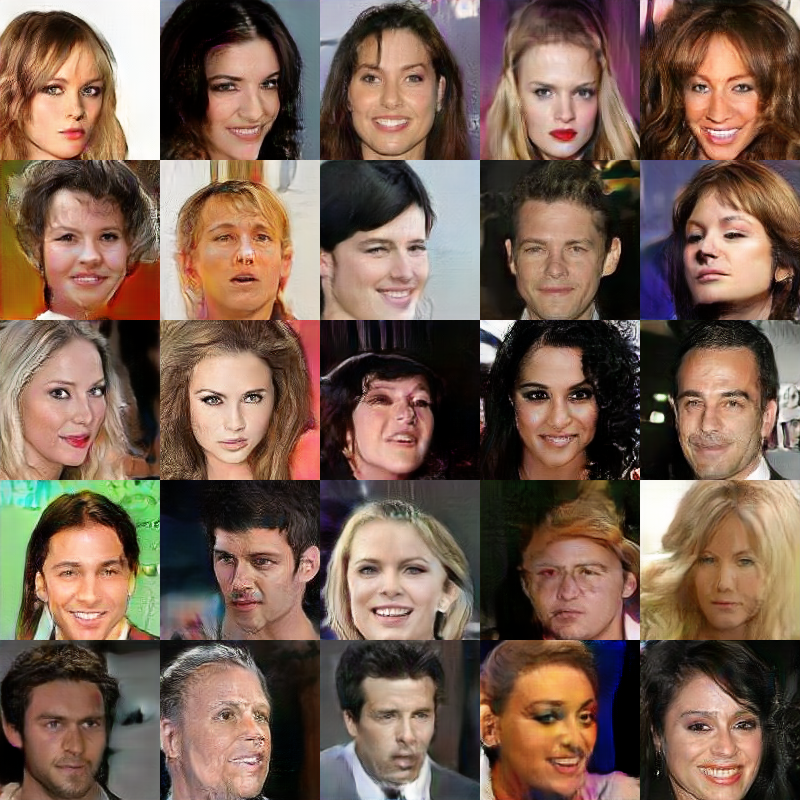
\includegraphics[width=.32\columnwidth]{samples/celeba-mmd-rq-25.png}
%      ~
%      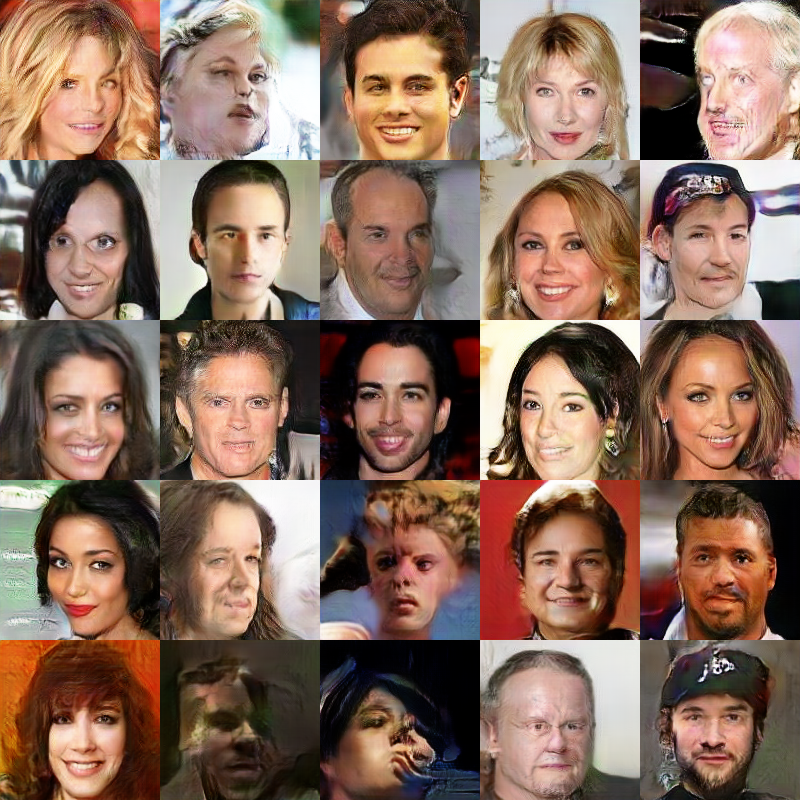
\includegraphics[width=.32\columnwidth]{samples/celeba-wgan-25.png}
%      ~
%      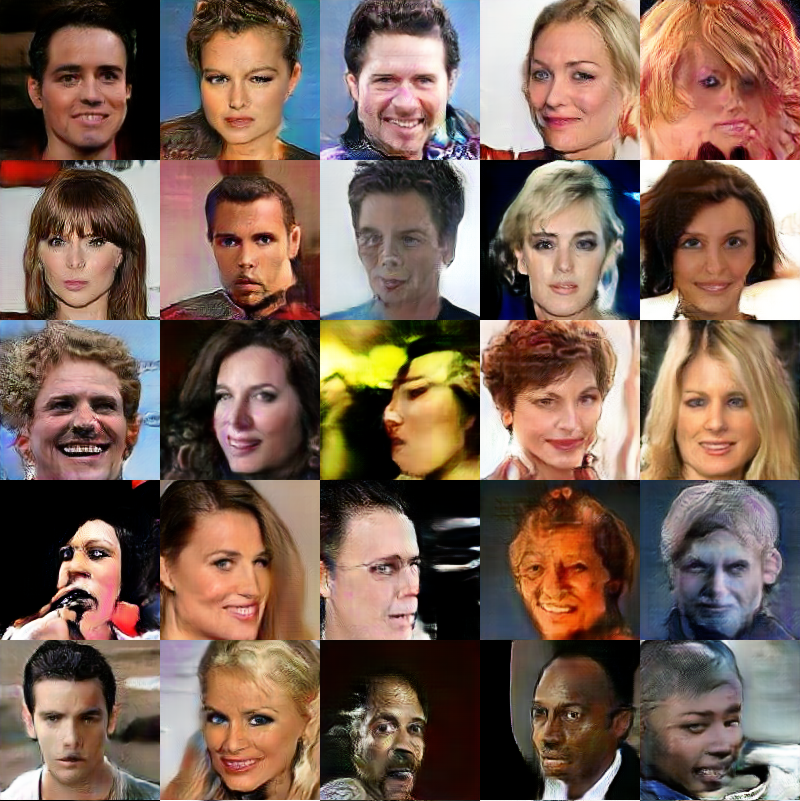
\includegraphics[width=.32\columnwidth]{samples/celeba-cramer-25.png}
%      \caption{Samples for \textbf{$160 \times 160$ CelebA} dataset trained with 
%               MMD GAN (left) and WGAN-GP (right) with ResNet generator and DCGAN discriminator.}
%    \end{figure}
    \begin{sidefigure4}
      \centering
      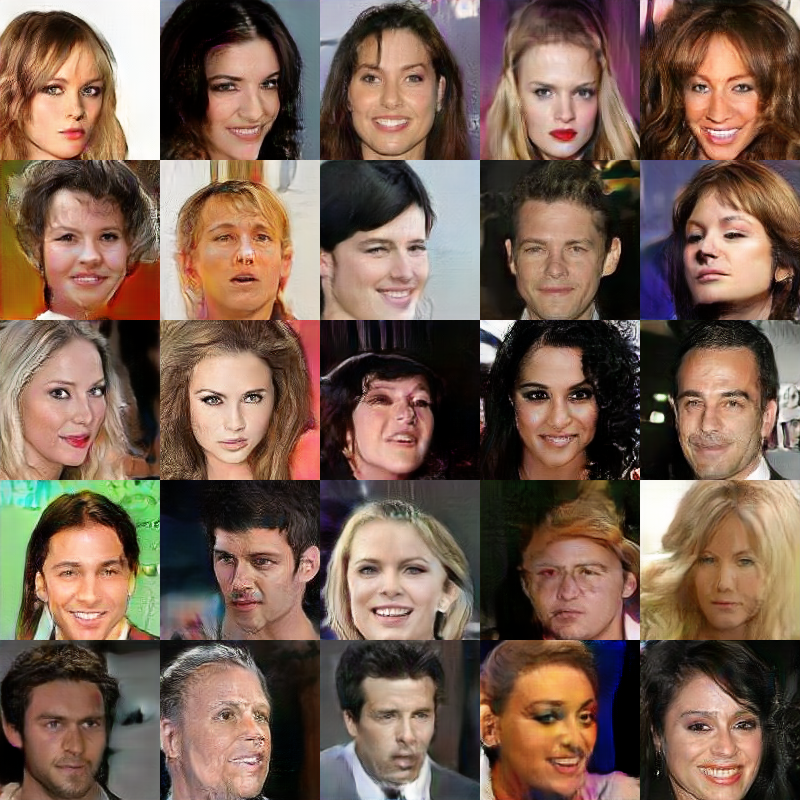
\includegraphics[width=.49\columnwidth]{samples/celeba-mmd-rq-25.png}
      ~
      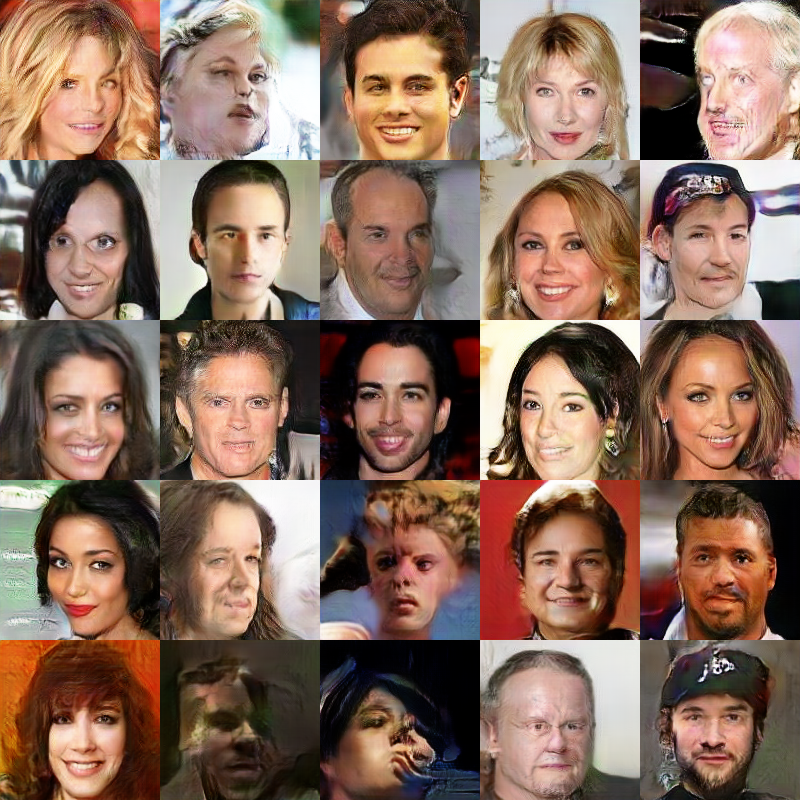
\includegraphics[width=.49\columnwidth]{samples/celeba-wgan-25.png}
      \vspace*{10pt}
      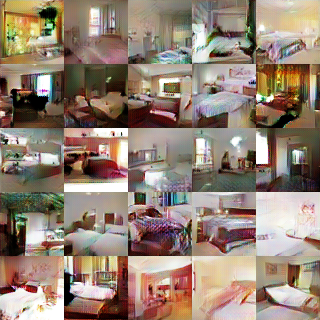
\includegraphics[width=.49\columnwidth]{samples/lsun_rq_16.png}
      ~
      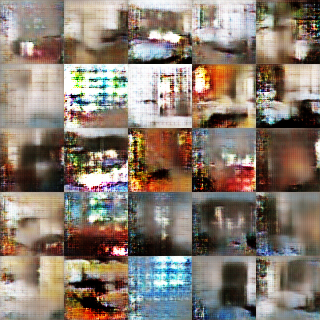
\includegraphics[width=.49\columnwidth]{samples/lsun_wgan_16.png}
      \caption{\textbf{$160 \times 160$ CelebA dataset.} \\
               Samples from
               MMD GAN (left) and WGAN-GP (right) trained with ResNet generator and DCGAN critic.\\
               \vspace*{95pt}
               \textbf{$64 \times 64$ LSUN bedroom dataset.}\\
               Samples from 
               MMD GAN (left) and WGAN-GP (right) models trained with DCGAN 
               architecture with \emph{small critic}\\ ($4\times$ less convolutional filters) .%\\[10pt]
               %MMD GANs trained with composite \emph{rational quadratic} kernel.
               }
    \end{sidefigure4}
    \vspace*{-1.3cm}
    \begin{table}
      \centering
      \vspace{-1cm}
      \caption{Mean (standard deviation) of score evaluations for the CelebA dataset.}
      \label{tab:celeba-scores}
      \begin{tabular}{cc|rrr}
        loss & top layer & \multicolumn{1}{c}{Inception} & \multicolumn{1}{c}{FID} & \multicolumn{1}{c}{KID} \\
        \hline
        MMD RQ   &   16 &    2.61  (0.01) &   20.55  (0.25) &   0.013  (0.001)\\
        Cram\'er &  256 &    2.86  (0.01) &   31.30  (0.17) &   0.025  (0.001)\\
        WGAN-GP  & 1    &    2.72  (0.01) &   29.24  (0.22) &   0.022  (0.001)\\
        test set & --   &    3.76  (0.02) &    2.25  (0.04) &   0.000  (0.000)\\
    \end{tabular}
\end{table}
  \end{column}

  \begin{column}{.32\textwidth}
    \begin{block}{KID - new evaluation method for GANs}
      \emph{Inception score} and \emph{Fr\'echet Inception Distance (FID)} are two common methods 
      of GAN evaluation. Yet, both have drawbacks. 
      \begin{itemize}
        \item Inception is independent of the target distribution and not meaningful for datasets such as LSUN or CelebA.
        \item FID estimates are biased.
        \item We propose an alternative method, \emph{Kernel Inception Distance (KID)}, defined as 
      MMD estimate (with kernel $k(x,y) = \left(\frac{1}{d}\langle x, y\rangle + 1\right)^3$)
      between Inception hidden layer activations of the samples. 
%        \item KID has low bias even for moderate sample sizes.
      \end{itemize}
    \end{block}
    \begin{figure}
      \centering
      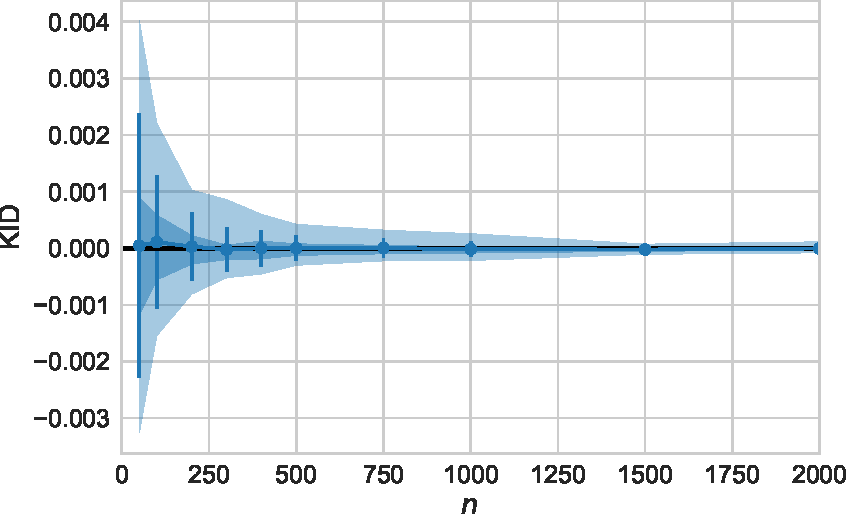
\includegraphics[width=.48\columnwidth]{figs/mmd-unbiased.pdf}\quad
      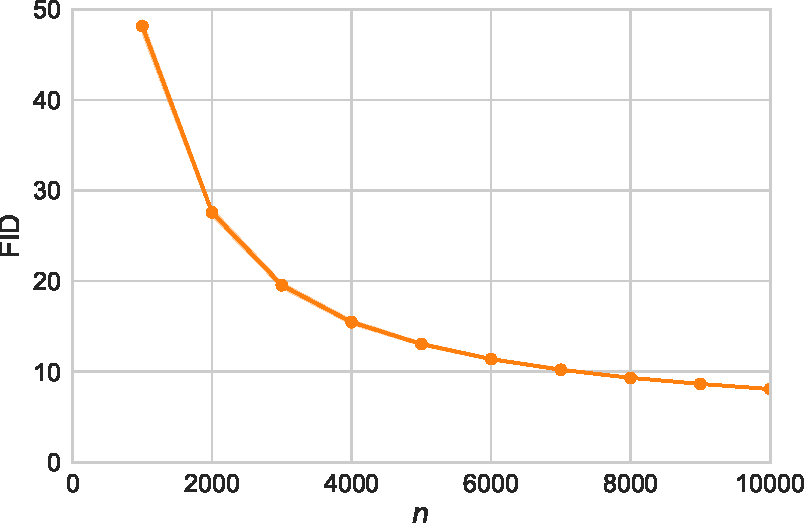
\includegraphics[width=.48\columnwidth]{figs/fid-bias.pdf}
      \caption{Estimates of KID (left) and FID (right) between the CIFAR-10 train and test sets. FID estimates 
        exhibit strong bias for $n$ even up to $10\,000$, which is not the case for KID. 
        Standard deviation of estimates shrinks quickly for KID and is always small for FID.}  %Each point is based on 100 samples, estimating with replacement; sampling without replacement, and/or using the full training set, gives similar results. Lines show means, error bars standard deviations, dark colored regions a $\frac{2}{3}$ coverage interval of the samples, light colored regions a $95\%$ interval. Note the differing $n$ axes.}
      \label{fig:fid-kid-bias}
    \end{figure}
    \begin{block}{Learning Rate Adaptation}
      \begin{itemize}
%        \item Decreasing learning rate is common in deep learning.
        \item In GAN training, learning rate is usually tuned by hand.
        \item We propose an adaptive scheme, based on comparing the KID score for samples from consecutive iterations.
      \end{itemize}
    \end{block}
     \printbibliography
  \end{column}

\end{columns}


\end{frame}


\end{document}
